% Copyright 2004 by Till Tantau <tantau@users.sourceforge.net>.
%
% In principle, this file can be redistributed and/or modified under
% the terms of the GNU Public License, version 2.
%
% However, this file is supposed to be a template to be modified
% for your own needs. For this reason, if you use this file as a
% template and not specifically distribute it as part of a another
% package/program, I grant the extra permission to freely copy and
% modify this file as you see fit and even to delete this copyright
% notice. 

\documentclass{beamer}

\usetheme{Madrid}
\usepackage[lithuanian]{babel}
\usepackage[utf8x]{inputenc}
\def\LTfontencoding{L7x}
% \PrerenderUnicode{ąčęėįšųūž}
\usepackage{times}
\usepackage[T1]{fontenc}
\usepackage{color}
\usepackage{verbatim}
\usepackage{graphicx}
\usepackage{fancyvrb}
\usepackage{bm}
\usepackage{amsfonts}
\usepackage{float}
\usepackage{hyperref}
\usepackage{LTPlius}

\usepackage{caption}
\usepackage{subfig}
\usepackage[T1]{fontenc}
\usepackage{tgtermes}

\usepackage{xcolor}
\definecolor{raudona}{RGB}{202,82,61}
\definecolor{zalia}{RGB}{133,181,98}
\definecolor{melyna}{RGB}{46,75,167}


\include{pythonlisting}

% \documentclass{beamer} --------idk

\usetheme{Madrid}
\usepackage{graphicx}
\usepackage{subfig}



\title{Dirbtinio intelekto modelių kolapsas}
\author{Greta Virpšaitė}
\institute[Vilniaus Universitetas]
{
\\
  Vilniaus universitetas
  \\
  Matematikos ir informatikos fakultetas
  \\
  Programų sistemų bakalauro studijų programa
  \\
}
\date{2025}



% Let's get started
\begin{document}

\begin{frame}
  \titlepage
\end{frame}


\begin{frame}{Pagrindiniai terminai}
    \textbf{Dirbtinio intelekto (DI) modelių kolapsas} - degeneratyvus procesas, kuris atsiranda, kai generatyviniai modeliai mokomi naudojant jų pačių sugeneruotus duomenis praranda gebėjimą tiksliai atspindėti pradinę duomenų informaciją.

%gilieji neuroniniai tinklai
\end{frame}


\begin{frame}{Pagrindiniai terminai}
     \begin{figure}[!htbp]
            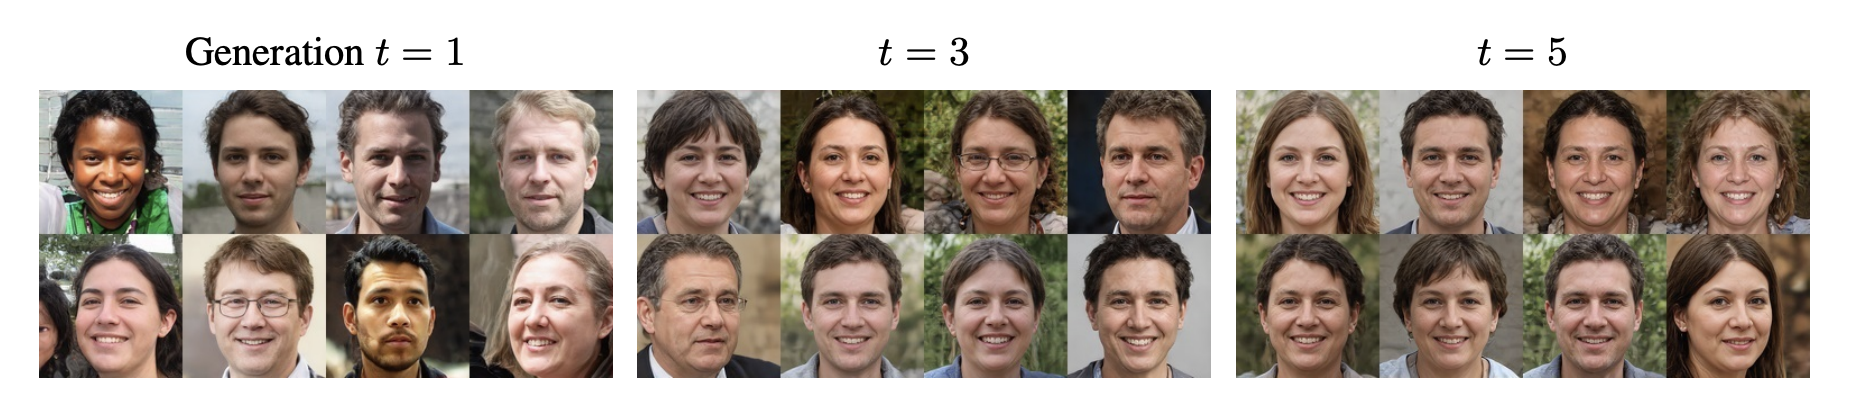
\includegraphics[width=1\textwidth]{images/nuotraukuKolapsas.png}
            \caption{\textbf{FFHQ-StyleGAN2 kolapso pavizdys.}
            Didėjant generacijų (angl. \textsl{Generation}) skaičiui \enquote{t} matomas išvesčių suvienodėjimas. }
            \label{fig:test_single_image}
    \end{figure}

%Nuotraukose galima pastebėti kaip keičiantis t (generacijų (angl. generations) skaičiui) modelio įvairovė nyksta. Tai atsispindi žmonių odos ir plaukų spalvų, emocijų, drabužių bei aplinkos įvairovės sumažėjime.
\end{frame}

\begin{frame}{Pagrindiniai terminai}
    \textbf{Save valgantys ciklai} - Mokymo ciklai, kurie parodo, kaip modelio mokymas su sugeneruotais duomenimis gali lemti kolapsą. Save valgantys ciklai priskiriami trims kategorijoms: Sintetinių duomenų ciklai, sintetinių augmentacijų ciklai ir ciklai su šviežiais duomenimis.
\end{frame}

\begin{frame}{Pagrindiniai terminai}
     \begin{figure}[!htbp]
            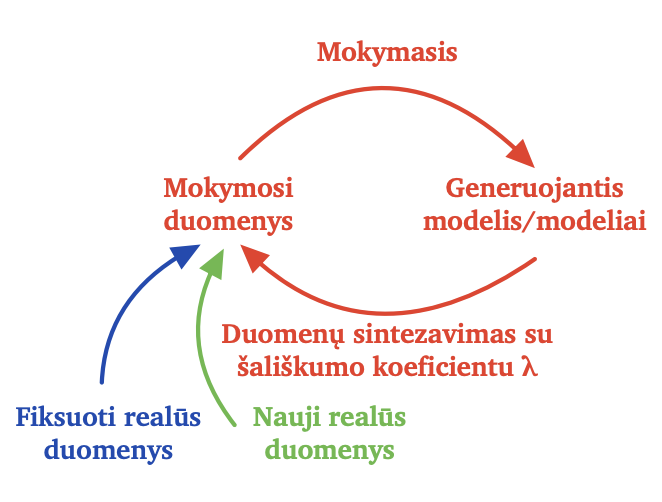
\includegraphics[width=0.5\textwidth]{images/valgantysCiklai.png}
            \caption{\textbf{Save valgančių ciklų iliustracija.}
                \begin{itemize}
                    \item \textbf{\textcolor{raudona}{Pilnai sintetinių duomenų ciklą}}: apibūdina ciklą, kuriame naudojami tik pilnai sintetiniai duomenys.
                \end{itemize}}
            \label{fig:test_single_image}
    \end{figure}
\end{frame}

\begin{frame}{Pagrindiniai terminai}
     \begin{figure}[!htbp]
            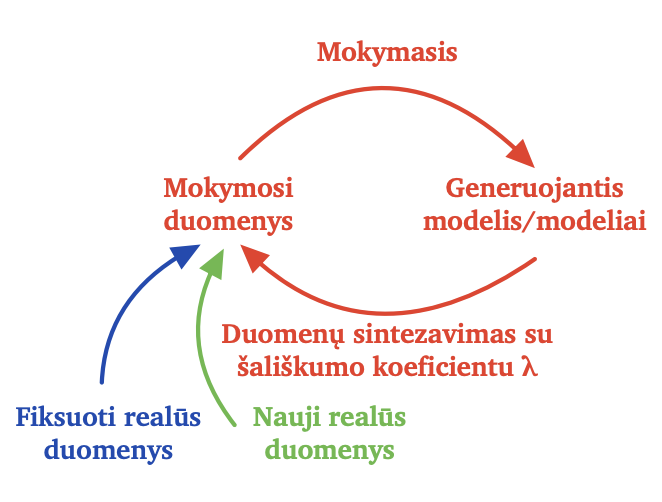
\includegraphics[width=0.5\textwidth]{images/valgantysCiklai.png}
            \caption{\textbf{Save valgančių ciklų iliustracija.}
                \begin{itemize}
                    \item \textbf{Sintetinių duomenų augmentacijų ciklą}: šiame cikle naudojami \textbf{\textcolor{melyna}{fiksuoti realūs duomenys}} kartu su \textbf{\textcolor{raudona}{pilnai sintetiniais duomenimis}}.
                \end{itemize}}
            \label{fig:test_single_image}
    \end{figure}
\end{frame}

\begin{frame}{Pagrindiniai terminai}
     \begin{figure}[!htbp]
            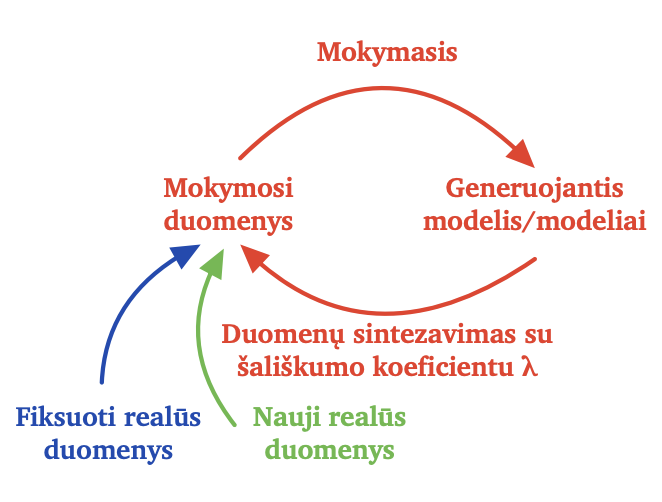
\includegraphics[width=0.5\textwidth]{images/valgantysCiklai.png}
            \caption{\textbf{Save valgančių ciklų iliustracija.}
                \begin{itemize}
                    \item \textbf{Ciklą su šviežiais duomenimis}: ciklas, apima \textbf{\textcolor{zalia}{naujus realius duomenis}} kartu su \textbf{\textcolor{raudona}{pilnai sintetiniais duomenimis}}.
                \end{itemize}}
            \label{fig:test_single_image}
    \end{figure}
\end{frame}

\begin{frame}{Pagrindiniai terminai}
     \begin{figure}[!htbp]
            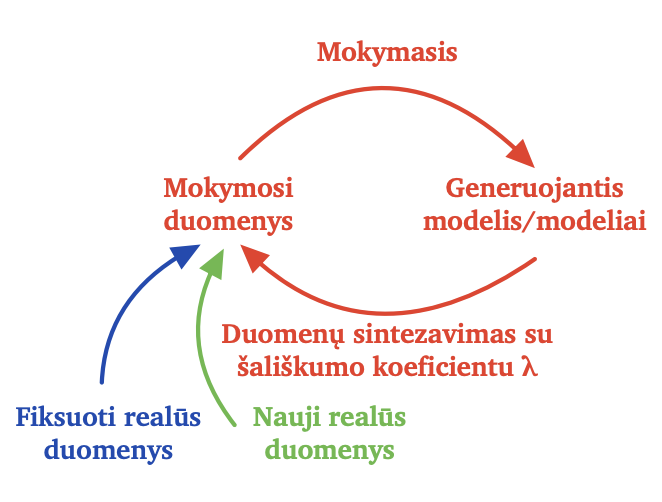
\includegraphics[width=0.5\textwidth]{images/valgantysCiklai.png}
            \caption{\textbf{Save valgančių ciklų iliustracija.}
                \begin{itemize}
                    \item  šališkumo parametras \textbf{\textcolor{raudona}{\(\lambda\)}} nusako, kaip atrodys generuojamų pavyzdžių kokybės ir įvairovės pasiskirstymas.
                \end{itemize}}
            \label{fig:test_single_image}
    \end{figure}
\end{frame}










% -------------------------------------------------
\begin{frame}{Tikslas}
\begin{itemize}
    \item Giliau išnagrinėti DI modelių kolapso mechanizmus,  šiuolaikinius mokslinius metodus, skirtus šios problemos identifikavimui ir sprendimui, su tikslu pateikti įžvalgas apie galimas prevencines priemones ir jų implementavimą kasdienėje praktikoje.
\end{itemize}

% \begin{enumerate}
%     \item Numeruojamo sąrašo pavyzdys
%     \item Sekančioje skaidrėje pateikiamas vu logotipas (žr. \ref{fig:vu logo}).
% \end{enumerate}
\end{frame}

% Uždaviniai - ----------------------------------

\begin{frame}{Uždaviniai}
\begin{itemize}
    \item Išanalizuoti literatūrą, susijusią su DI modelių kolapsu, apimant pagrindinius mechanizmus, rizikas ir galimus sprendimus. Aprašyti DI modelių kolapso atpažinimo technikas, remiantis šiuolaikiniais tyrimais.
    \item Apibrėžti pagrindines DI modelių kolapso prevencijos strategijas, įtraukiant Europos Sąjungos DI aktą ir jo įtaką DI modelių stabilumui.
\end{itemize}
\end{frame}

\begin{frame}{Uždaviniai}
\begin{itemize}
    \item Atlikti eksperimentą su VAE modeliu, mokant jį MNIST duomenų rinkiniu, siekiant ištirti modelio kolapso reiškinį.
    \\
    \item Aptarti etines implikacijas, susijusias su DI modelių kolapsu ir jo prevencija.
    \\
    \item Parengti rekomendacijas, pagrįstas atliktos analizės rezultatais, kurios galėtų būti pritaikomos moksliniuose ir praktiniuose kontekstuose.
\end{itemize}
\end{frame}

\begin{frame}{Eksperimentas}
    \textbf{Kodėl pasirinktas VAE neuroninio tinklo architektūra?}
    \begin{itemize}
        \item Paprastos architektūros, kolapsui iliustruoti tinkamas tinklas, kurio veikimo mechanizmai aprašyti nagrinėjamoje mokslinėje literatūroje.
        \item Leidžia vizualiai stebėti modelio išvesčių pokyčius skirtingose treniravimo strategijose.
    \end{itemize}

    \textbf{Kodėl pasirinktas MNIST duomenų rinkinys?}
    \begin{itemize}
        \item Plačiai naudojamas kaip pavyzdinis duomenų rinkinys dirbtinio intelekto modelių mokymui.
        \item MNIST buvo naudotas viename iš nagrinėtų tyrimų, kitame - analizuotas \(\lambda\) koeficiento poveikis kolapsui, o šiame tyrime tiriamas ciklo tipo parinkties efektas.
    \end{itemize}
\end{frame}


% ---------------------------------------------
\begin{frame}{Rezultatai}
     \textbf{Sintetinių duomenų ciklas:}
        \begin{itemize}
            \item Po penktosios generacijos VAE modelis parodė stiprų kolapso efektą: prarastos daugelio skaitmenų įvairovės savybės.
            \item Tik keli skaitmenys (0, 3, 6, 8, 9) buvo atpažįstami, tačiau ir jie buvo labai blankūs.
        \end{itemize}
\end{frame}

\begin{frame}{Rezultatai}
    \begin{figure}[!htbp]
        \subfloat[][Pirma genereracija]{
            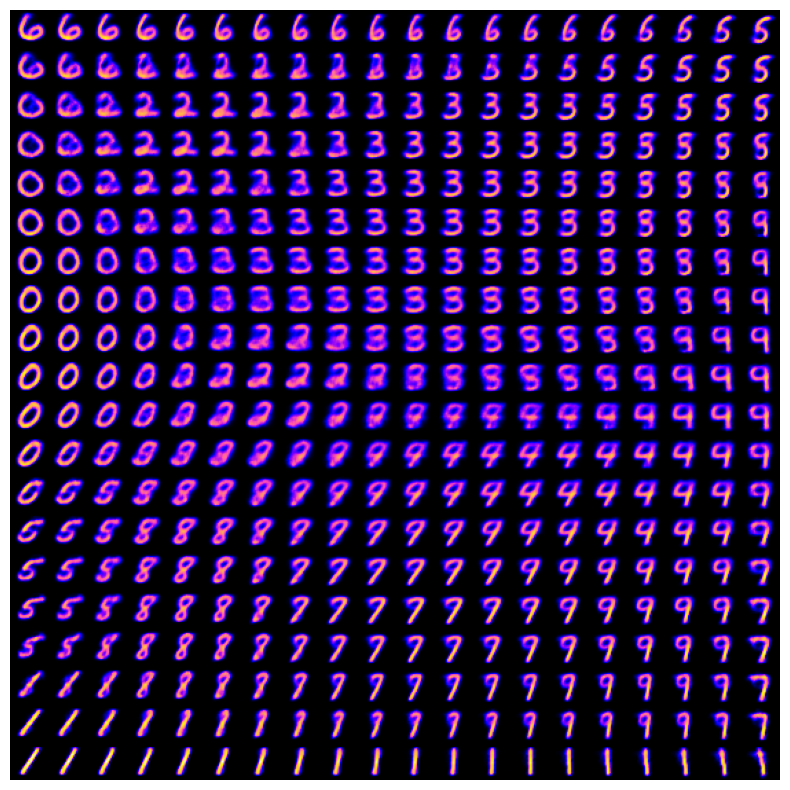
\includegraphics[width=0.45\textwidth]{images/synthetic_generation_1.png}
            \label{fig:synthetic_gen_1}
        }
        \hfill
        \subfloat[][Penkta genereracija]{
            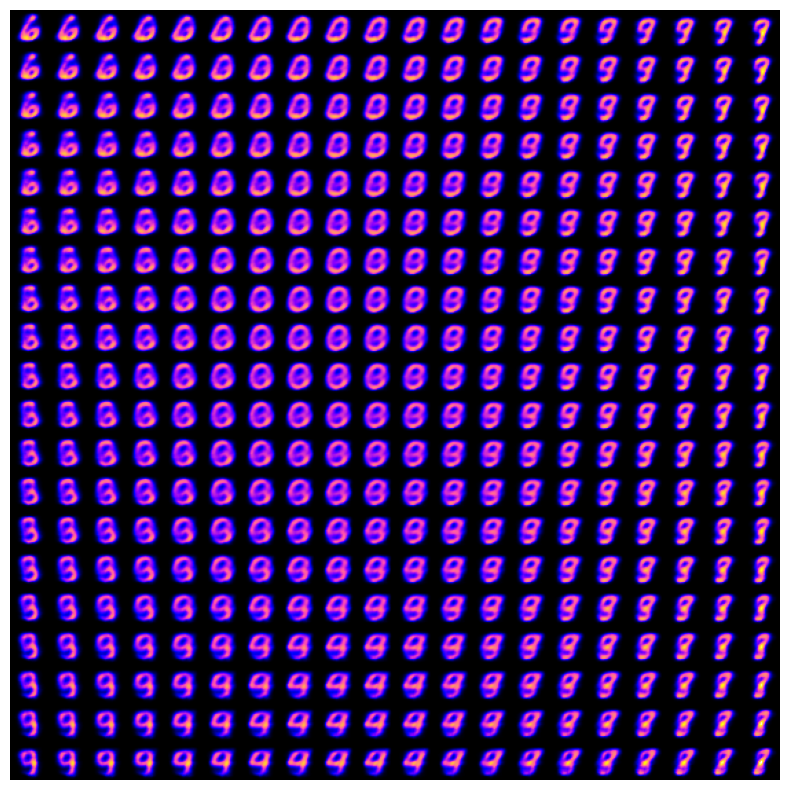
\includegraphics[width=0.45\textwidth]{images/synthetic_generation_2.png}
            \label{fig:synthetic_gen_2}
        }
        \caption{Pirmosios ir penktosios sintetinių duomenų ciklo generacijos palyginimas.}
        \label{fig:comparison_generations}
    \end{figure}
\end{frame}




\begin{frame}{Rezultatai}
   \textbf{Sintetinių augmentacijų ciklas:}
        \begin{itemize}
            \item Vizualiai rezultatų kokybė nuo pirmos iki penktos generacijos žymiai nesiskyrė.
            \item Pastebėtas nežymus vaizdų suliejimas.
        \end{itemize}
\end{frame}

\begin{frame}{Rezultatai}
    \begin{figure}[!htbp]
        \subfloat[][Pirma genereracija]{
            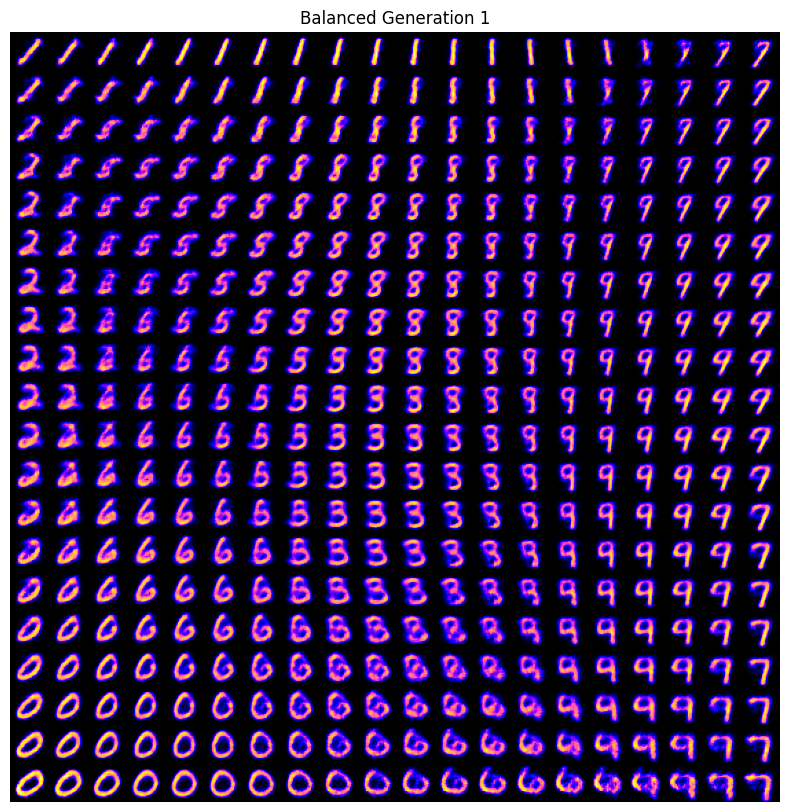
\includegraphics[width=0.45\textwidth]{images/real_synthetic_generation_1.png}
            \label{fig:real_synthetic_gen_1}
        }
        \hfill
        \subfloat[][Penkta genereracija]{
            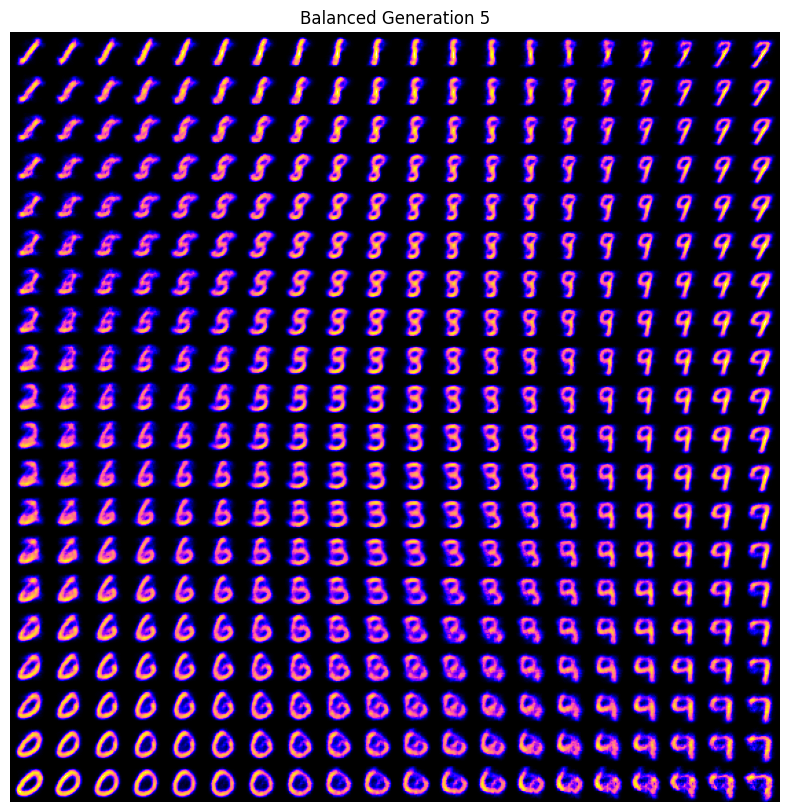
\includegraphics[width=0.45\textwidth]{images/real_synthetic_generation_5.png}
            \label{fig:real_synthetic_gen_2}
        }
        \caption{Pirmosios ir penktosios sintetinių augmentacijų ciklo generacijos palyginimas.}
        \label{fig:comparison_generations}
    \end{figure}
\end{frame}

\begin{frame}{Rezultatai}
    \begin{itemize}
        \item \textbf{Ciklas su šviežiais duomenimis:}
        \begin{itemize}
            \item Po penktos generacijos tinklo išvestys tapo šiek tiek ryškesnės.
            \item Įvairovės praradimas nebuvo pastebėtas.
        \end{itemize}
    \end{itemize}
\end{frame}

\begin{frame}{Rezultatai}
    \begin{figure}[!htbp]
        \subfloat[][Pirma genereracija]{
            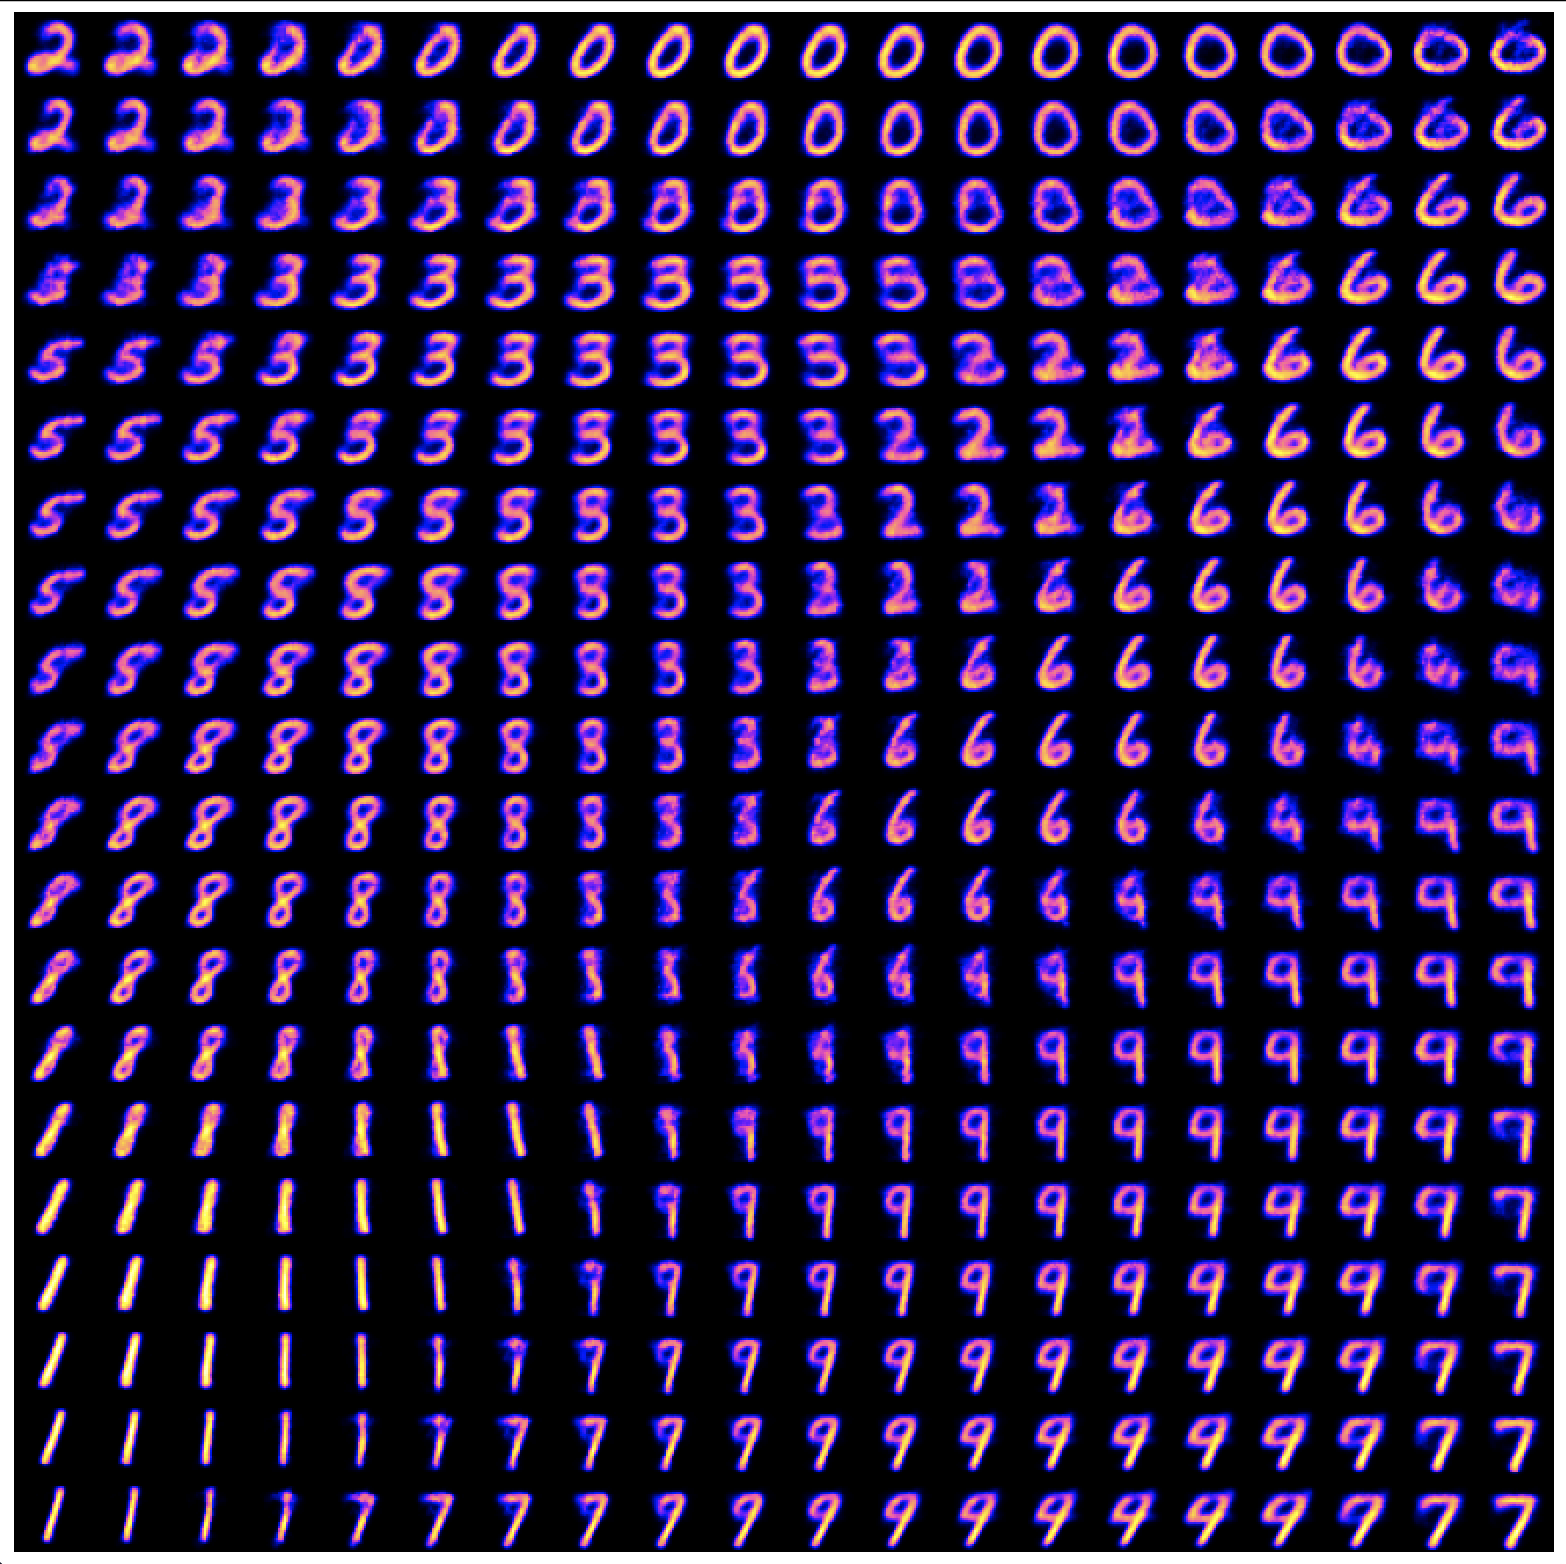
\includegraphics[width=0.45\textwidth]{images/fresh_generation_1.png}
            \label{fig:synthetic_gen_1}
        }
        \hfill
        \subfloat[][Penkta genereracija]{
            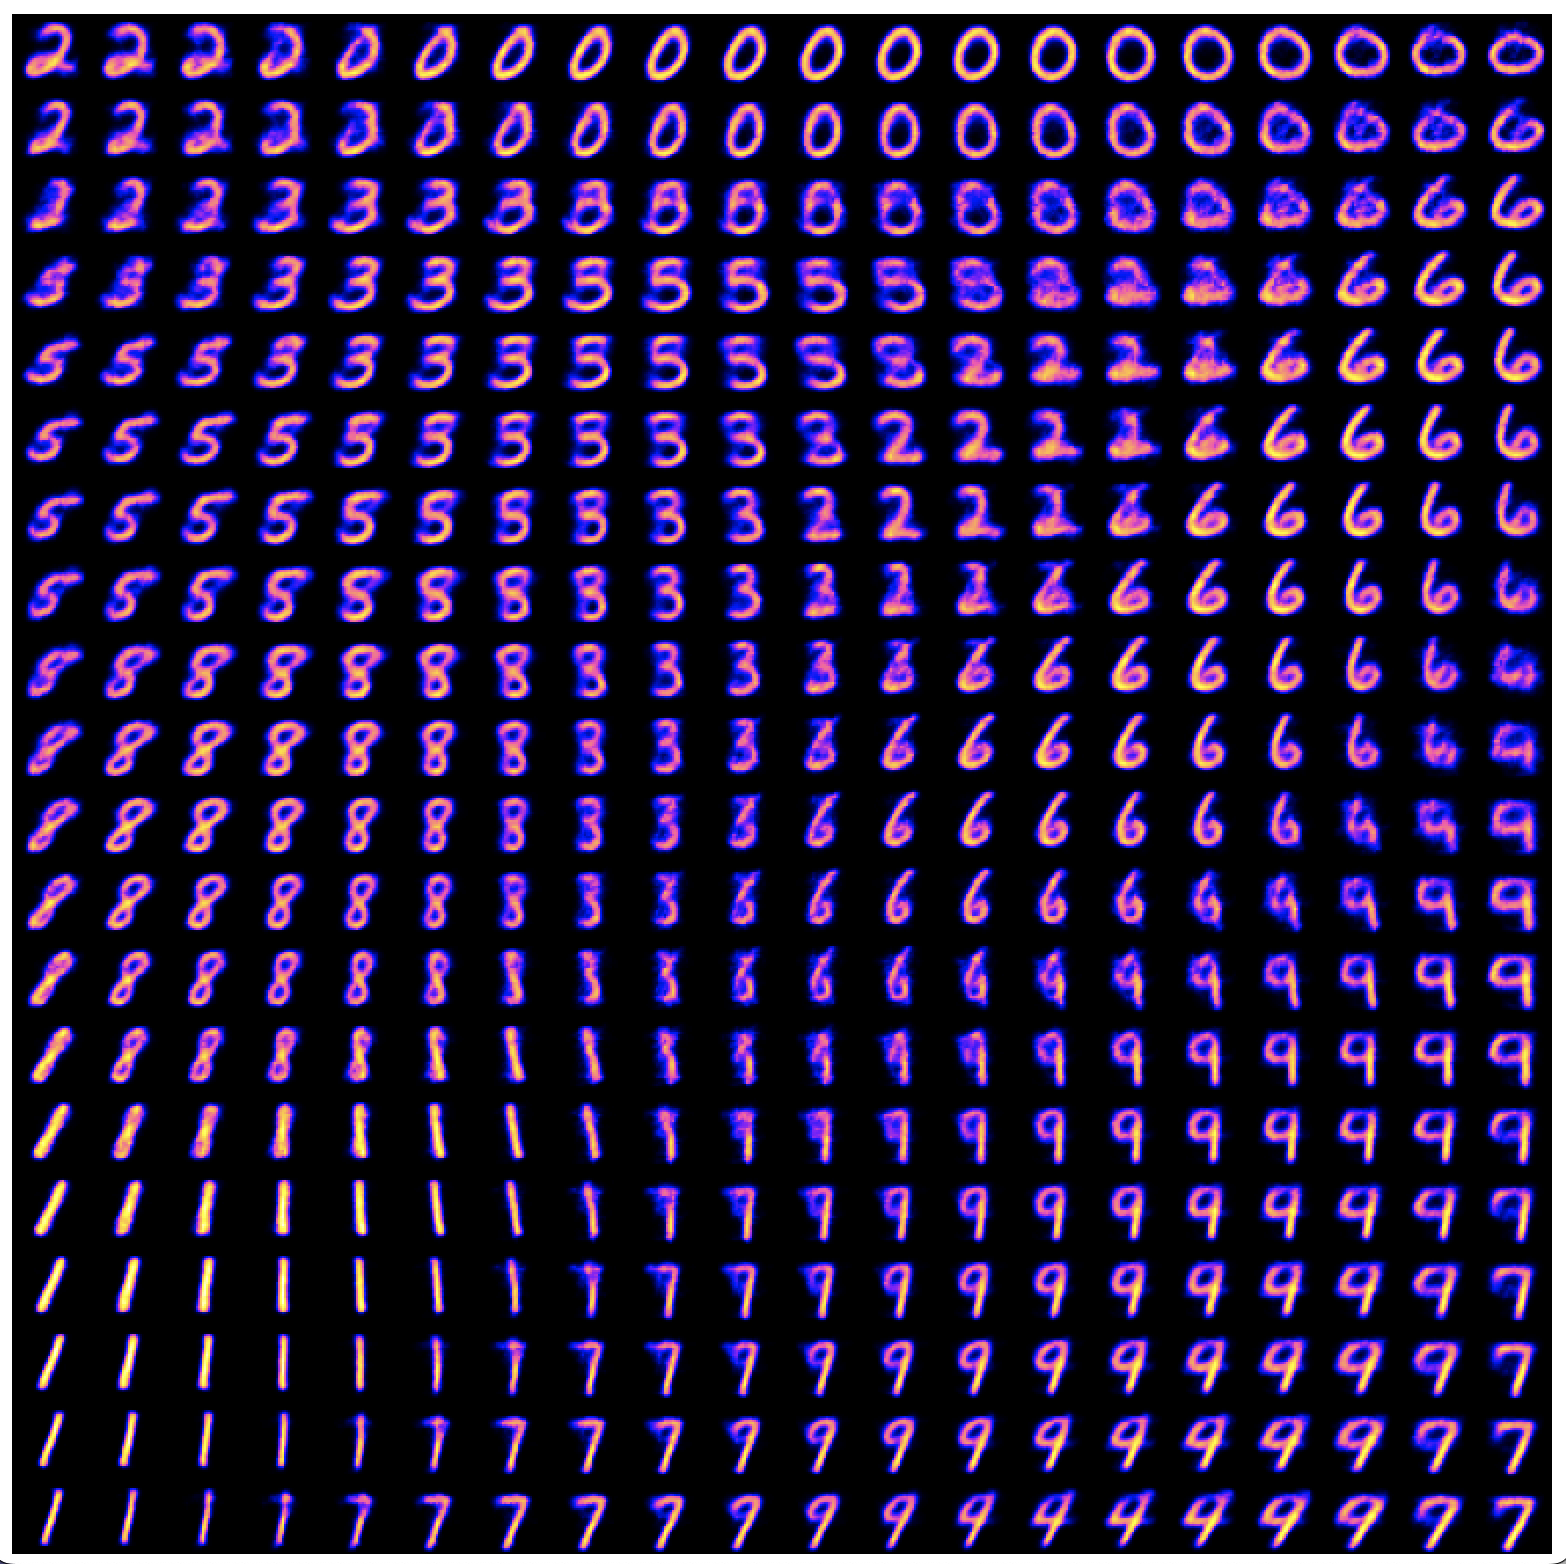
\includegraphics[width=0.45\textwidth]{images/fresh_generation_5.png}
            \label{fig:synthetic_gen_2}
        }
        \caption{Pirmosios ir penktosios ciklo su šviežiais duomenimis generacijos palyginimas.}
        \label{fig:comparison_generations}
    \end{figure}
\end{frame}

\begin{frame}{Rezultatai}
   \textbf{Standartinio modelio mokymas:}
        \begin{itemize}
            \item Po penktos generacijos duomenų kokybė pagerėjo, vaizdai tapo ryškesni ir aiškesni.
            \item Modelis parodė gebėjimą mokytis.
        \end{itemize}
\end{frame}

\begin{frame}{Rezultatai}
    \begin{figure}[!htbp]
        \subfloat[][Pirma genereracija]{
            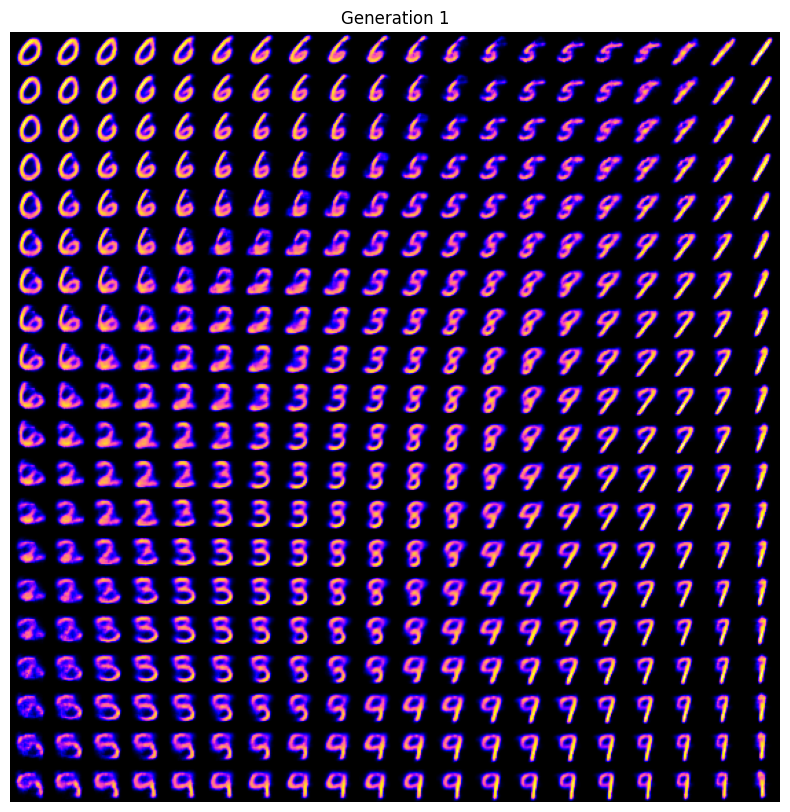
\includegraphics[width=0.45\textwidth]{images/original_generation_1.png}
            \label{fig:synthetic_gen_1}
        }
        \hfill
        \subfloat[][Penkta genereracija]{
            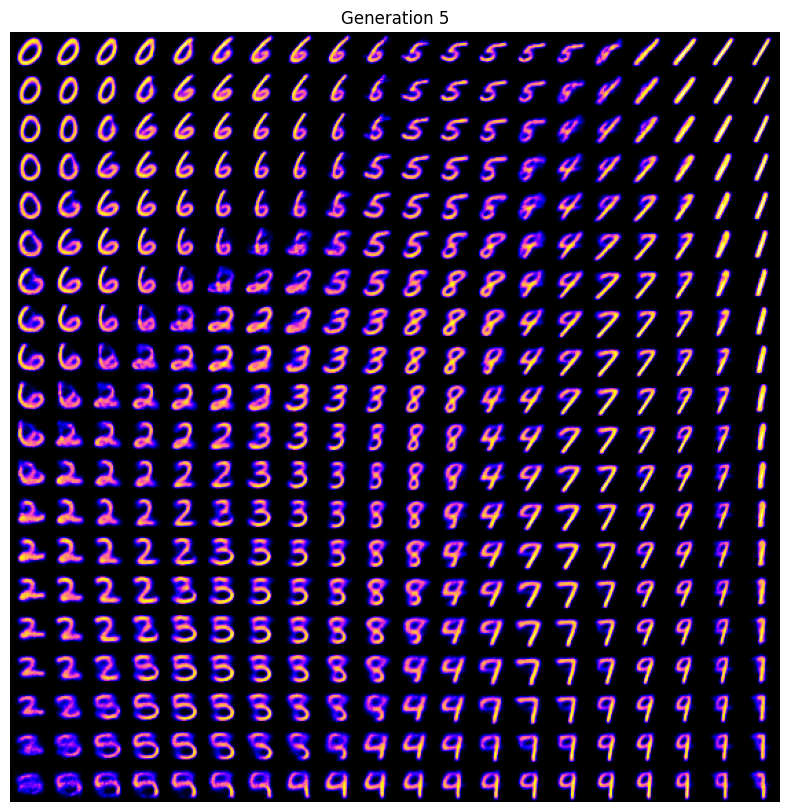
\includegraphics[width=0.45\textwidth]{images/original_generation_5.png}
            \label{fig:synthetic_gen_2}
        }
        \caption{Pirmosios ir penktosios generacijų su standartiniu apmokymu palyginimas}
        \label{fig:comparison_generations}
    \end{figure}
\end{frame}

%---------------------------------------------------------


\begin{frame}{Išvados}
    \item \textbf{DI modelių kolapso pobūdis:}
    \begin{itemize}
        \item DI modelių kolapsas atsiranda, kai modeliai mokomi naudojant jų pačių sugeneruotus duomenis, o tai lemia duomenų įvairovės praradimą.
        \item Eksperimentai patvirtino, kad kolapsas sintetinių duomenų cikluose yra neišvengiamas ir pasireiškia jau po kelių generacijų.
    \end{itemize}
\end{frame}

\begin{frame}{Išvados}
    \textbf{Maišymo strategijos efektyvumas:}
            \begin{itemize}
                \item Realių ir sintetinių duomenų maišymas (augmentacijos ir šviežių duomenų cikluose) sumažina kolapso riziką, tačiau netinkamas santykis šviežių duomenų cikluose gali sukelti kokybės praradimus, o sintetinių augmentacijų cikluose tik nutolinti Di modelių kolapsą.
                \item Naujų realių duomenų įtraukimas į mokymo procesą išlieka efektyviausiu būdu mažinti kolapso riziką.
            \end{itemize}
\end{frame}



\begin{frame}{Išvados}
    \textbf{Reguliavimo svarba:}
        \begin{itemize}
            \item Europos Sąjungos DI reglamentas, apimantis duomenų žymėjimą ir šališkumo kontrolę, gali netiesiogiai padėti DI modeliams išvengti kolapso.
            \item Reglamentas įsigalios tik 2026 metais, todėl kolapso prevencijai būtina plėtoti alternatyvius sprendimus iki to laiko.
        \end{itemize}
\end{frame}

\begin{frame}{Rekomendacijos}
   
        \textbf{Mokslininkams:} 
        
        \begin{itemize}
            \item Rekomenduojama tęsti tyrimus, siekiant geriau suprasti sintetinių ir šviežių realių duomenų santykio poveikį DI modelių stabilumui bei jų kokybei.
            \item Gilintis į šališkumo kontrolės parametro \(\lambda\) reikšmę skirtingose generatyvinėse architektūrose ir mokymosi cikluose.
            \item tyrinėti ilgalaikį sugeneruotų duomenų maišymo poveikį tarp skirtingų modelių ir jų rezultatų kokybę
        \end{itemize}

   
\end{frame}


\begin{frame}{Rekomendacijos}
     \textbf{Praktikams:}
     \begin{itemize}
         \item Užtikrinti, kad duomenų rinkiniai būtų reguliariai atnaujinami šviežiais realiais duomenimis
         \item Užtikrinti, kad sintetiniai duomenys būtų naudojami subalansuotai, neviršijant saugių proporcijų
     \end{itemize}
\end{frame}

\begin{frame}{Rekomendacijos}
    \textbf{Politikos kūrėjams ir vykdytojams:}
    \begin{itemize}
        \item Siūloma Europos Sąjungos DI akte toliau stiprinti reikalavimus sugeneruotų duomenų žymėjimui ir kontrolės mechanizmams.
        \item Svarstyti įtraukti daugiau nuostatų, skirtų mažesnės rizikos DI sistemoms.
        \item Valdomiesiems kūnams kurti ir kitus reglamentus ar įstatymus skirtus DI kolapso mažinimo tematikai
    \end{itemize}
\end{frame}

\begin{frame}{Rekomendacijos}
     \textbf{Bendruomenei:} 
        \begin{itemize}
            \item Didinti informuotumą apie DI modelių kolapso rizikas ir jų prevencijos svarbą.
            \item Atkreipti dėmesį į tai, kaip sistemų naudotojai prisideda prie duomenų kokybės, ir skatinti juos neteršti interneto modelių sugeneruotais duomenimis
        \end{itemize}
\end{frame}
% \section{LaTeX konstrukcijų pavyzdžiai}
% \subsection{Sąrašai}
% \begin{frame}{Sąrašai}
% \begin{itemize}
%     \item Nenumeruojamo sąrašo pavyzdys
%     \item Antras punktas
% \end{itemize}

% \begin{enumerate}
%     \item Numeruojamo sąrašo pavyzdys
%     \item Sekančioje skaidrėje pateikiamas vu logotipas (žr. \ref{fig:vu logo}).
% \end{enumerate}
% \end{frame}



% \section{LaTeX konstrukcijų pavyzdžiai}
% \subsection{Sąrašai}
% \begin{frame}{Sąrašai}
% \begin{itemize}
%     \item Nenumeruojamo sąrašo pavyzdys
%     \item Antras punktas
% \end{itemize}

% \begin{enumerate}
%     \item Numeruojamo sąrašo pavyzdys
%     \item Sekančioje skaidrėje pateikiamas vu logotipas (žr. \ref{fig:vu logo}).
% \end{enumerate}
% \end{frame}

% \subsection{Paveiksliukai}
% \begin{frame}{Paveiksliuko įterpimo pavyzdys}
% \begin{figure}[!htbp]
%     \includegraphics[scale=0.43]{vu_logo}
%     \label{fig:vu logo}

%     \caption{VU logotipas}
% \end{figure}
% \end{frame}


% \begin{frame}{Dviejų paveiksliukų įterpimo pavyzdys}
% \begin{figure}[!htbp]
% \subfloat[][Pirmojo paveiksliuko pavadinimas]{
%     \includegraphics[width=0.33\textwidth]{vu_logo}
%     \label{fig:pirmojo paveiksliuko id}
% }
% \subfloat[][Antrojo paveiksliuko pavadinimas]{
%     \includegraphics[width=0.33\textwidth]{vu_logo}
%     \label{fig:antrojo paveiksliuko id}
% }
% \caption{Bendras abiejų paveiksliukų pavadinimas}
% \label{fig:paveiksliuku pavyzdzio id}
% \end{figure}
% \end{frame}


% \subsection{Python kodo fragmento pavyzdys}
% \begin{frame}[fragile]{Python kodo framgmento įterpimo pavyzdys}
% % Python kodo fragmentus galima įterpti štai taip:
% Šis fragmentas yra ne 2 kart 2 o, 2 pakelta kvadratu:
% \begin{python}
% >>> 2**2
% 4
% \end{python}
% \end{frame}


% \appendix
% \section<presentation>*{\appendixname}
% \subsection<presentation>*{For Further Reading}

% \begin{frame}[allowframebreaks]
%   \frametitle<presentation>{Šaltiniai}
%   \begin{thebibliography}{10}
    
%   \beamertemplatebookbibitems

%   \bibitem{Author1990}
%     Mano ypatingas svarbus šaltinis
%     \newblock {\url{http://python.org/dev/peps/pep-0008}}.
 
%   \end{thebibliography}
% \end{frame}

\end{document}







% \begin{frame}{Test Single Image}
%     \begin{figure}[!htbp]
%         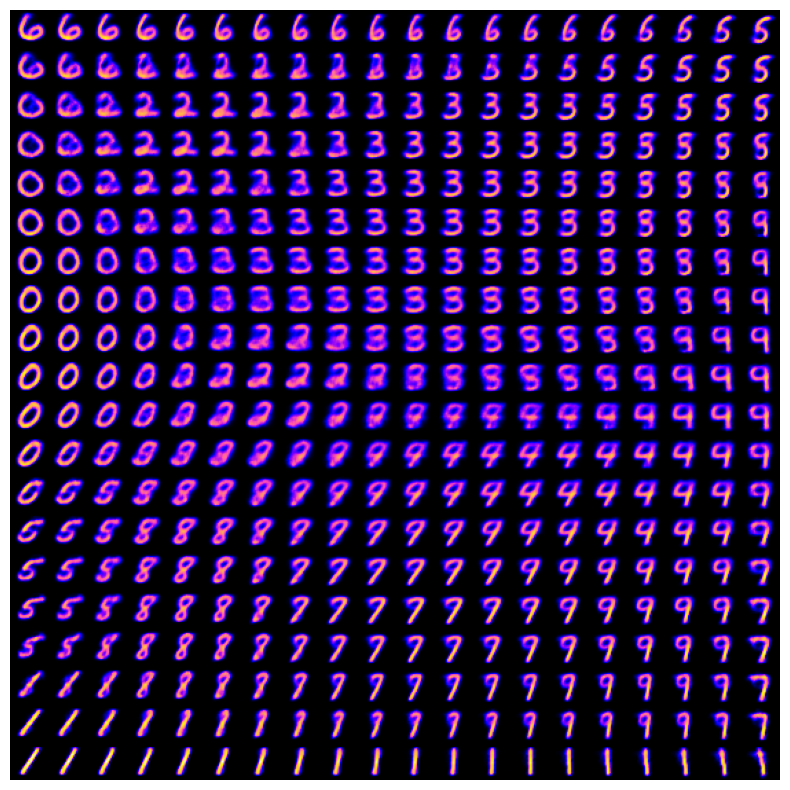
\includegraphics[width=0.5\textwidth]{images/synthetic_generation_1.png}
%         \caption{Test of a Single Image}
%         \label{fig:test_single_image}
%     \end{figure}
% \end{frame}

% \begin{frame}{Test Two Images Side-by-Side}
%     \begin{figure}[!htbp]
%         \subfloat[][First Image: Generation 1]{
%             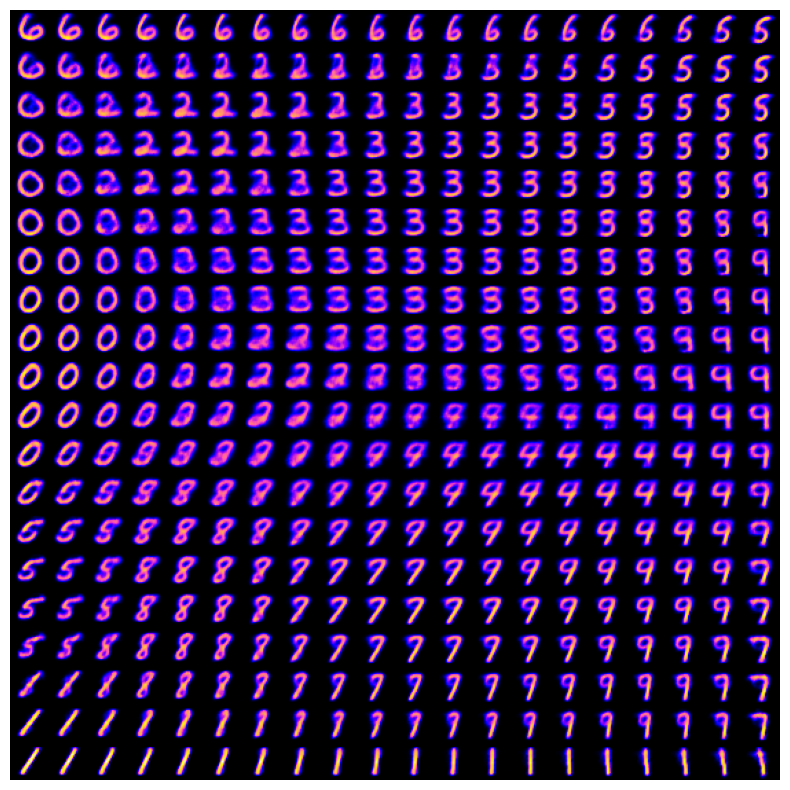
\includegraphics[width=0.45\textwidth]{images/synthetic_generation_1.png}
%             \label{fig:synthetic_gen_1}
%         }
%         \hfill
%         \subfloat[][Second Image: Generation 2]{
%             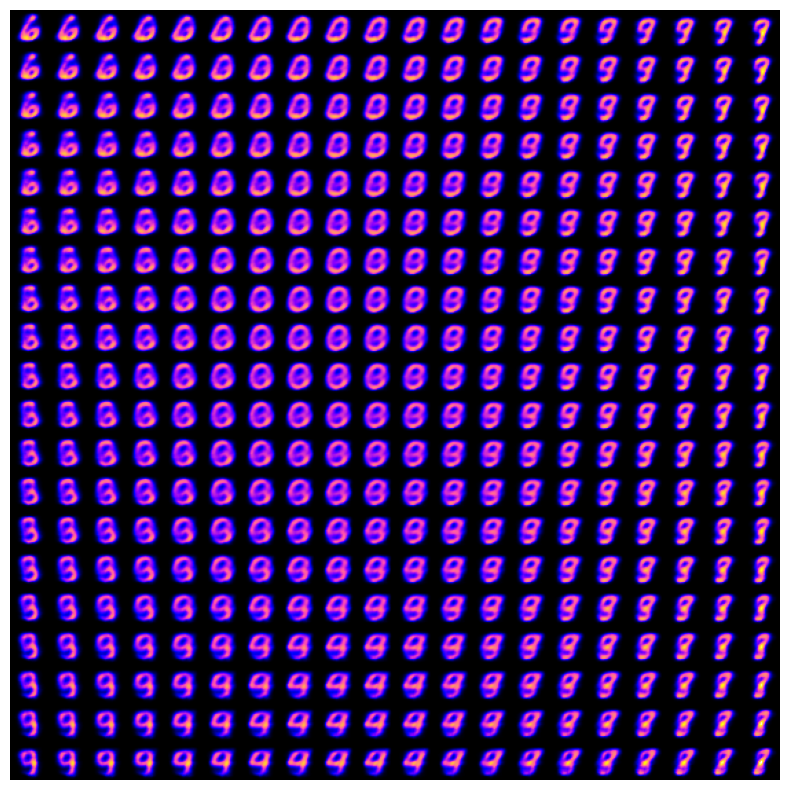
\includegraphics[width=0.45\textwidth]{images/synthetic_generation_2.png}
%             \label{fig:synthetic_gen_2}
%         }
%         \caption{Comparison of Generation 1 and Generation 2}
%         \label{fig:comparison_generations}
%     \end{figure}
% \end{frame}


